\documentclass[final]{sig-alternate-05-2015}

\usepackage{url}                  % format URLs
\usepackage{listings}          % format code
\lstset{
  mathescape, 
  language={C},
  basicstyle=\small
}
\usepackage{enumitem}      % adjust spacing in enums
\usepackage[colorlinks=true,allcolors=blue,breaklinks,draft=false]{hyperref}   
\usepackage{graphicx}
\usepackage{float}
\usepackage{subcaption}
\usepackage{xspace,framed}
\usepackage{colortbl}
\usepackage{calc}
\usepackage[dvipsnames]{xcolor}
\usepackage{amssymb,amsmath,amsfonts} 
\usepackage{mathtools}
\usepackage{microtype}

\usepackage{algorithm}
\usepackage{amsfonts}
\usepackage{multicol}
\usepackage{multirow}
\usepackage{tikz}
\usetikzlibrary{positioning, automata, shapes.arrows, calc, shapes, arrows}
\usetikzlibrary{patterns}
\usepackage[justification=centering]{caption}
\usepackage{stmaryrd}
\usepackage{hhline}
\usepackage{pifont}
\usepackage{longtable}
\usepackage{afterpage}
\usepackage{wasysym}
\usepackage[scaled]{helvet}

\newcommand{\blue}[1]{{\color{blue}#1}}
\newcommand{\red}[1]{{\color{red}#1}}
\newcommand{\green}[1]{{\color{green}#1}}

\newtheorem{myassumption}{Assumption}
\newtheorem{mylemma}{Lemma}
\newtheorem{myprop}{Proposition}

\renewcommand{\baselinestretch}{0.99}
\allowdisplaybreaks
\newcommand{\lcsay}[1]{{\color{Magenta} LC: {#1}}} 
\newcommand{\dcsay}[1]{{\color{purple} DC: {#1}}}
\newcommand{\dksay}[1]{{\color{blue} DK: {#1}}}  
\newcommand{\aasay}[1]{{\color{red} AA: {#1}}} 
\newcommand{\cdsay}[1]{{\color{Mahogany} CD: {#1}}} 
\newcommand{\pksay}[1]{{\color{RoyalBlue} PK: {#1}}} 
\newcommand{\ibsay}[1]{{\color{Sepia} IB: {#1}}} 

\newcommand{\param}[2]{\ensuremath{\langle{#1},{#2}\rangle}\xspace}


\begin{document}

\CopyrightYear{2017}
\setcopyright{acmcopyright}
\conferenceinfo{HSCC '17,}{April 18--20, 2017, Pittsburgh, PA, USA.}
\isbn{978-1-4503-4590-3/17/04}\acmPrice{\$15.00.}
\doi{TBD.}

\title{
Sound and Automated Synthesis of Digital Stabilizing Controllers for Continuous
Plants%
\thanks{Supported by EPSRC grant EP/J012564/1,
ERC project 280053 (CPROVER) and the H2020 FET OPEN SC$^2$.}}

\author{Alessandro Abate$^{1}$, Iury Bessa$^{2}$, Dario Cattaruzza$^{1}$, Lucas Cordeiro$^{1,2}$, \\ 
Cristina David$^{1}$, Pascal Kesseli$^{1}$ and Daniel Kroening$^{1}$
\and
$^{1}$\affaddr{University of Oxford, Oxford, United Kingdom} \\
$^{2}$\affaddr{Federal University of Amazonas, Manaus, Brazil}
}


\newcommand\tool{{\sf DSSynth}\xspace}

\maketitle

\begin{abstract}
%
Modern control is implemented with digital microcontrollers, embedded within
a dynamical plant that represents physical components. Correct control is
non-trivial, however. The problem is exacerbated by artefacts specific to digital
control, such as the effects of finite-precision arithmetic, time discretization,
and quantization noise introduced by A/D and D/A conversion.  Thus, the
programming is a key barrier to broad adoption of digital control, and requires
considerable expertise.
%
We present a new algorithm based on Counter-Example Guided Inductive
Synthesis (CEGIS) that automates the design of digital controllers for a given
continuous plant model that are correct by construction. This approach
promises to reduce the cost and time of development of digital control
dramatically, and requires considerably less expertise than methodologies
driven by verification. Specifically, we soundly
synthesize controllers for hybrid closed-loop systems, i.e., software-implemented
embedded controllers along with a model of their physical environment (the plant),
that are \emph{stable}, taking into consideration the effects of time-discretization
(sampling), quantization (A/D and D/A converters), and the use of finite-precision arithmetic.

\paragraph{Problem Statement}
We only consider linear transfer function models, and require a $z$-domain transfer
function $G(z)$ that captures all aspects of the continuous plant with a
Laplace domain transfer function $G(s)$ and the sampling and hold process. 
The continuous model of the plant must be discretized to obtain the
corresponding coefficients of $G(z)$.

Given a synchronized ZOH input and sample-and-hold output on the plant with
a sample time $T$ satisfying the Nyquist criterion, the discrete pulse
transfer function $G(z,T)$ is an exact z-domain representation of $G(s)$
that can be computed using the following formula:
%
\begin{equation}
\label{eq:pulsetf}
G(z,T) = (1-z^{-1})\mathcal{Z}\left\lbrace{\mathcal{L}^{-1}\left\lbrace{\frac{G(s)}{s}}\right\rbrace_{t=kT}}\right\rbrace.
\end{equation}
%
For the sake of brevity, we will use the notation $G(z)$ to represent $G(z,T)$.

We further consider parametric errors (tolerances) in the plant model such that
\begin{equation}
\label{eq:tolerancetf}
\hat{G}(z) = G(z)+\Delta_pG(z).
\end{equation}
Due to the nature of the methods we use for the stability check, we require
that the parametric errors in the plant have the same polynomial order as
the plant itself, since tolerances of higher order would invalidate
feedback model.

Finally we consider the discretization effect of modelling the plant using Fixed Precision arithmetic
\begin{equation}
\label{eq:fwltf}
\tilde{G}(z) = \mathcal{F}\langle I,F\rangle(\hat{G}(z))
\end{equation}

Where $\mathcal{F}\langle I,F\rangle(\cdot)$ is a discretizing function that truncates the coefficients of $\hat{G}(z)$ using $I$ integer bits and $F$ fractional bits. This last effect does not exist in the actual implementation, but it is caused by the use of fixed precision arithmetic in the synthesis and verification tools.
The controller model has no tolerances and is already aligned with the Fixed Precision arithmetic, thus $\tilde{C}(z)=\hat{C}(z)=C(z)$. Notice that this is a condition on the synthesiser, which must ensure these equalities are met.
The effects of the A/D, D/A quantizations are introduced as bounded additive uncertainties ($\nu_1(z),\nu_2(z)$) that need to be stabilized along with the plant. These sources are assumed to be non-deterministic, 
which poses no further restriction to our model. Notice that the quantization noise is additive, which means
it does not affect the transfer function.

The overall closed loop equation describing the system in figure \ref{fig:sampledsystem} becomes.
\begin{equation}
\tilde{Y}(z)=\nu_{1}(z)+\tilde{G}(z) \tilde{C}(z) R(z)+\tilde{G}(z)\nu_{2}(z)-\tilde{G}(z) \tilde{C}(z) \tilde{Y}(z)
\end{equation}
which will be stable if the poles in $\frac{1}{1+\hat{G}(z)\hat{C}(z)}$ remain within the unit circle.
We use Jury's Criterion~\cite{astrom1997computer} to ensure this, thus avoiding the calculation of polynomial roots.
The resulting closed-loop
system is a program loop that operates on bit-vectors encoded using
fixed-point arithmetic with finite word length (FWL).  The deterministic
effects of the FWL and quantization errors are incorporated into the model
as an additive uncertainty, which is taken into account during the
CEGIS-based synthesis of the control software for the plant.

\paragraph{Our Synthesis Approach}
We have implemented our new algorithm in a tool called \tool, and are able
to automatically generate stable controllers for a set of intricate plant
models taken from the literature within minutes.
The tool uses a two stage approach. 
As the cost of SAT solving increases with in the size of the problem
instance, our algorithm tries to solve the problem first for small word length,
iteratively increasing the precision if it is insufficient.
The initial phase uses SAT-solving
techniques in order to synthesise a candidate solution. This solution is neither sound nor universal.
The candidate is then fed to a formal verifier, which will prove its universality for the collection of plant models (considering the tolerances). If the verifier finds a counterexample, it will be fed back to the synthesiser, which will use it as a guideline for future synthesis, thus slicing away candidate solutions that are not likely to be universal. If no counter-example is found by the verifier, it enters a second phase in which it restores soundness by evaluating the result using interval arithmetic. If this check fails, the loop returns to the synthesis phase, requiring higher precision in order to minimise rounding errors. If the check passes, we have found a sound stabilizing controller.
%
\end{abstract}


\printccsdesc

\begin{figure*}[htb]
\centering

\tikzset{add/.style n args={4}{
    minimum width=6mm,
    path picture={
        \draw[circle] 
            (path picture bounding box.south east) -- (path picture bounding box.north west)
            (path picture bounding box.south west) -- (path picture bounding box.north east);
        \node[draw=none] at ($(path picture bounding box.south)+(0,0.13)$)     {\small #1};
        \node[draw=none] at ($(path picture bounding box.west)+(0.13,0)$)      {\small #2};
        \node[draw=none] at ($(path picture bounding box.north)+(0,-0.13)$)    {\small #3};
        \node[draw=none] at ($(path picture bounding box.east)+(-0.13,0)$)     {\small #4};
        }
    }
 }

\resizebox{1.0\textwidth}{!}{
 \begin{tikzpicture}[scale=0.6,-,>=stealth',shorten >=.2pt,auto,
     semithick, initial text=, ampersand replacement=\&,]

  \matrix[nodes={draw, fill=none, shape=rectangle, minimum height=.2cm, minimum width=.2cm, align=center}, row sep=.6cm, column sep=.6cm] {
    \node[draw=none] (r) {$R(z)$};
%   \& \coordinate (aux0);
   \& \node[circle,add={-}{+}{}{}] (circle) {};
   \node[draw=none] (ez) at ([xshift=1cm,yshift=.15cm]circle)  {$e(z)$};
   \& \node[rectangle,draw,
	minimum width=1cm,
	minimum height=1cm,
        label=\textbf{Controller}] (cz) {{\sc C(z)}};
   \node[draw=none] (ud) at ([xshift=1cm,yshift=.15cm]cz)  {$U(z)$};
     
   \& complexnode/.pic={ 
      \node[rectangle,draw,
	minimum width=3cm,
	minimum height=1.6cm,
	label=\textbf{DAC},] (dac) {};
     \node[circle,add={}{+}{+}{},fill=gray!20] (q2) at ([xshift=-.65cm]dac.center) {};
     \node[draw=none] (q2t)  at ([xshift=-.65cm,yshift=-.65cm]dac.center) {{\sc Q2}};
     \node[draw=none] (v2)  at ([xshift=-.65cm,yshift=1.5cm]dac.center) {$\nu_2(z)$};
     \node[fill=gray!20] (zoh) at ([xshift=.65cm]dac.center) {{\sc ZOH}};}   
   \& \node[rectangle,draw,
	minimum width=1cm,
	minimum height=1cm,
        label=\textbf{Plant}] (gs) {{\sc $\hat{G}(s)$}};
   \node[draw=none] (ud) at ([xshift=-2cm,yshift=.15cm]gs)  {$U(s)$};
   \node[draw=none] (y) at ([xshift=2cm,yshift=.15cm]gs)  {$Y(s)$};
   \& complexnode/.pic={ 
     \node[rectangle,draw,
	minimum width=4cm,
	minimum height=1.6cm,
	label=\textbf{ADC},] (adc) {};
   \draw[] ([xshift=-1cm]adc.center) -- ++(0.5,0.2cm);
   \coordinate (switch1) at ([xshift=-1cm]adc.center);
   \coordinate (switch2) at ([xshift=-0.4cm]adc.center);
   \node[circle,add={}{+}{+}{},fill=gray!20] (q1) at ([xshift=1cm]adc.center) {};} 
     \node[draw=none] (q2t)  at ([xshift=1cm,yshift=-.65cm]adc.center) {{\sc Q1}};
   \node[draw=none] (v1)  at ([xshift=1cm,yshift=1.5cm]adc.center) {$\nu_1(z)$};
   \& \coordinate (aux1);
   \& \node[draw=none] (yz) {$\tilde {Y}(z)$};\\
   \& \coordinate (aux3); 
   \&
   \&
   \& 
   \& 
   \& \coordinate (aux2);\\
  };


  \path[->] (v1) edge (q1.north);
  \path[->] (v2) edge (q2.north);
  \path[->] (r) edge (circle.west);
  \path[->] (aux1) edge (yz);
  \path  
   (circle.east) edge (cz)
   (cz.east) edge (q2.west)
   (q2.east) edge (zoh.west)
   (zoh.east) edge (gs.west)
   (switch2) edge (q1.west)
   (q1.east) edge (aux1.west)
   (gs.east) edge (switch1.west)
   (aux1.south) edge (aux2.north)
   (aux2.west) edge (aux3.east); 
  \path[->]  (aux3.north) edge (circle.south);
 \end{tikzpicture}
}
 \caption{Closed-loop digital control system\label{fig:sampledsystem}}
\end{figure*}

\paragraph{Architecture of the Program Synthesizer}
\label{synthesizer-general}
%
The input specification provided to the program synthesizer is of the form
$\exists \vec{P} .  \forall \vec{x}.  \sigma(\vec{x}, \vec{P})$ where
$\vec{P}$ ranges over functions, $\vec{x}$ ranges over ground terms and
$\sigma$ is a quantifier-free formula.  We interpret the ground terms over
some finite domain $\mathcal{D}$.

The design of our synthesizer is given in Figure~\ref{fig:CEGIS} and consists
of two phases, {\sc Synthesize} and {\sc Verify}, which interact via a
finite set of test vectors {\sc inputs} that is updated incrementally. 
Given the aforementioned specification $\sigma$, the {\sc synth} procedure
tries to find an existential witness $\vec{P}$ satisfying the specification
$\sigma(\vec{x}, \vec{P})$ for all $\vec{x}$ in {\sc inputs} (as opposed to
all $\vec{x} \in \mathcal{D}$).
%
If {\sc synthesize} succeeds in finding a witness~$\vec{P}$, this witness
is a candidate solution to the full synthesis formula.  We pass this
candidate solution to {\sc verify}, which checks whether it is a full
solution (i.e., $\vec{P}$ satisfies the specification $\sigma(\vec{x},
\vec{P})$ for all $\vec{x}\in\mathcal{D}$).
%
If this is the case, then the algorithm terminates.  Otherwise, additional
information is provided to the {\sc synthesize} phase in the form of a new
counterexample that is added to the {\sc inputs} set and the loop iterates
again.

%
\begin{figure*}[htb]
\centering
%\resizebox{1\textwidth}{!}
{
 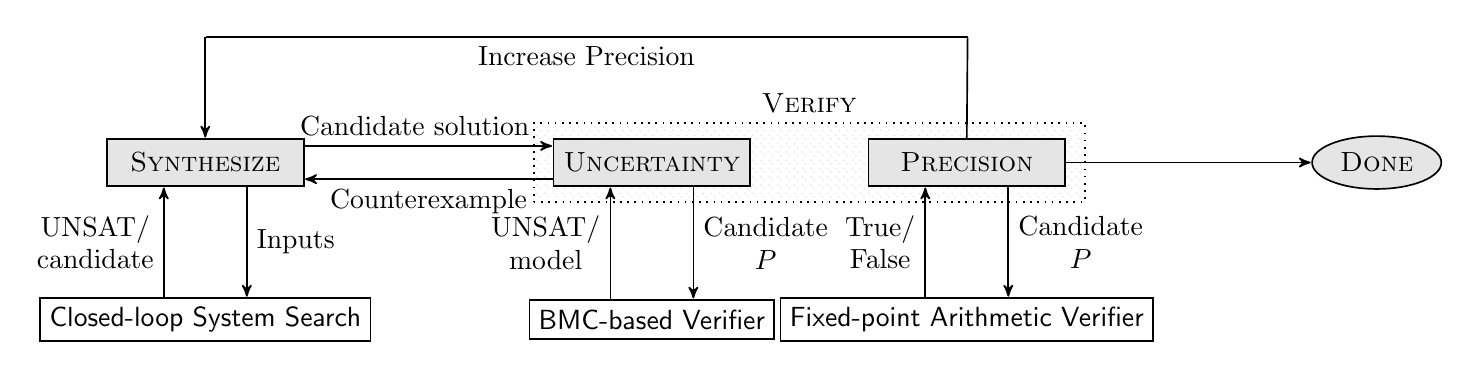
\begin{tikzpicture}[scale=0.3,->,>=stealth',shorten >=.2pt,auto, semithick, initial text=, ampersand replacement=\&,]
  \matrix[nodes={draw, fill=none, shape=rectangle, minimum height=.2cm, minimum width=.2cm, align=center
},
          row sep=.6cm, column sep=2cm] {
   \coordinate (aux1);
   \& \coordinate (aux2);
   \&;\\
   \node[minimum width=2.5cm, minimum height=0.6cm, fill=gray!20] (synth) {{\sc Synthesize}};
   \&
   complexnode/.pic={ 
     \node[rectangle,draw,dotted,
	minimum width=7cm,
	minimum height=1cm,
        pattern=north west lines, pattern color=gray!20,
	label={\sc Verify},] (verif) {};
     \node[minimum width=2.5cm, minimum height=0.6cm, fill=gray!20] (verif1) at ([xshift=-2cm]verif.center) {{\sc Uncertainty}};
     \node[minimum width=2.5cm, minimum height=0.6cm, fill=gray!20] (verif2) at ([xshift=2cm]verif.center) {{\sc Precision}};
   } 
   \& \node[ellipse, fill=gray!20] (done) {{\sc Done}};\\
   %% \node[fill=yellow!20] (verif) {{\sc ~~~~~~Uncertainty~~~~~~}};
   %% \&
   %% \node[fill=yellow!20] (verif2) {{\sc ~~~~~~Precision~~~~~~~}};\\
   \& \\
   \node[minimum height=0.5cm] (gp) {\sf Closed-loop System Search};
   \&
   complexnode/.pic={ 
     \coordinate (aux);
   \node[minimum height=0.5cm] (bmc) at ([xshift=-2cm]aux.center) {\sf BMC-based Verifier};
   \node[minimum height=0.5cm] (fp)  at ([xshift=2cm]aux.center) {\sf Fixed-point Arithmetic Verifier};
   }   
    \\
  };

   \path
    ([yshift=2em]synth.east) edge node[xshift=-0.5em] {Candidate solution} ([yshift=2em]verif1.west)
    ([yshift=-2em]verif1.west) edge node {Counterexample} ([yshift=-2em]synth.east)
    ([xshift=5em]verif1.south) edge node[align=center] {Candidate\\ $P$} ([xshift=5em]bmc.north)
    ([xshift=5em]verif2.south) edge node[align=center] {Candidate\\ $P$} ([xshift=5em]fp.north)
    ([xshift=-5em]bmc.north) edge node[align=center]  {UNSAT/\\model} ([xshift=-5em]verif1.south)
    ([xshift=-5em]fp.north) edge node[align=center]  {True/\\False} ([xshift=-5em]verif2.south)
    (verif2) edge node {} (done)
    ([xshift=5em]synth.south) edge node[align=center] {Inputs} ([xshift=5em]gp.north)
    ([xshift=-5em]gp.north) edge node[align=center] {UNSAT/\\candidate} ([xshift=-5em]synth.south)
    (aux1) edge (synth.north);
   \path[-]
   (verif2.north) edge node[align=center] {} ([xshift=6.7cm]aux2)
   ([xshift=6.7cm]aux2) edge node[align=center] {Increase Precision} (aux1);

 \end{tikzpicture}
}
\caption{Counterexample-Guided Inductive Synthesis of Closed-loop Systems
\label{fig:CEGIS}}
\end{figure*}
%

%%%%%%%%%%%%%%%%%%%%%%%%%%%%%%%%%%%%%%%%%%%%%%%%%%%%%%%%%%%%%%%%%%%%%%%%%%%%%%%%%%%%%%
\paragraph{Experimental Evaluation}\label{sec:experiments}

The median run-time amounts to $48$\,s, implying that \tool can synthesize half of the controllers 
in less than one minute. We consider these times short enough to be of practical use to control
engineers.  We further observe that the approach is able to synthesize stable controllers
in $20$ out of the $23$ benchmarks.  For the remaining benchmarks
our approach failed to synthesize a stable controller within the time
limits.  This can be addressed by either increasing either the time limit
or the fixed-point word widths considered, or by using floating-point
arithmetic instead.  The synthesized controllers were confirmed to be stable
outside of our model representation using MATLAB.

\bibliographystyle{abbrv}
\bibliography{paper}  

\end{document}
